\documentclass[numeric]{anvil-paper}
\usepackage{tikz}
\usepackage{pgfplots}
\usepgfplotslibrary{groupplots}
\pgfplotsset{compat=1.17}

\newcommand{\F}{\mathbb{F}}
\newcommand{\code}[1]{\texttt{#1}}
\newtheorem{proposition}{Proposition}

\title{Parity Words and Grid Shares:\\ Error-Correcting Mnemonics and Secret Sharing\\ over the BIP39 Wordlist}
\author{Robb Walters}
\date{November 2026}

\begin{document}
\maketitle

\begin{abstract}
A secret that no vendor can reset has to be copied onto paper or metal by hand
and read back years later. BIP39 mnemonics detect a copying mistake but cannot
repair one, and splitting a secret with Shamir's scheme multiplies the number of
hand-copied artefacts. We observe that a BIP39 word is already one symbol of the
field with 2048 elements, and put both error correction and threshold sharing
in that field. A phrase with $k$ appended Reed--Solomon \emph{parity words}
recovers from $e$ wrong and $s$ unreadable words whenever $2e+s\le k$, and from
swapped, dropped and extra words by a small edit search; the original mnemonic
is unchanged. Sharing such phrases word by word gives \emph{grid shares}: any
$t$ of $n$ cards recover the secret, fewer reveal nothing, every card repairs
itself, and spare cards repair each other when the cards are decoded together
(\emph{joint decoding}). In fault injection on a Lean~4
implementation, with one word in ten wrong, joint decoding recovered 99.5\% of
secrets from all five cards of a 3-of-5 set where repairing cards separately
recovered 31\%, and 61\% against 41\% from all three cards of a 2-of-3 set.
With exactly $t$ cards joint decoding adds nothing and reliability comes from
$k$ alone. In 31{,}600 trials the decoder returned no wrong secret.
\end{abstract}

\section{Introduction}
\label{sec:intro}

Shares of a secret can repair themselves and each other, at the level where
people make mistakes: whole words. That is the claim of this paper. It rests on
one observation. The BIP39 wordlist~\citep{bip39} has $2048 = 2^{11}$ entries,
so a written word is one element of the finite field $\F_{2^{11}}$, and both
tools a backup format needs are linear algebra over a field. Reed--Solomon
codes~\citep{reed1960polynomial} add redundancy within one written phrase.
Shamir's scheme~\citep{shamir1979how} spreads a secret over several phrases.
When both use the same field and the same symbols they compose into a product
code, and the result is decoded as one object.

The problem is practical. A 256-bit key with no reset path must be stored in
full, by its owner, for years, and the copies are made and read by hand. We
know of no published measurement of word error rates in hand-copied mnemonics.
The nearest evidence is about recall from memory: in a controlled study, 40\%
of participants could not reproduce an assigned 12-word BIP39 phrase after
three days and 49\% could not after seven. Of the 41 participants who failed,
14 had entered a phrase that the authors could in principle recover by bounded
search, and each of those was one wrong word, or one wrong word plus a change
of order~\citep{ambati2026notall}. Failures of
this kind are near misses. BIP39's checksum (4 bits for 12 words, 8 for 24)
says that such a phrase is wrong and nothing about where. Splitting the secret
raises the stakes: a 3-of-5 sharing has five phrases to copy, and deployed
formats decode each share separately (Section~\ref{sec:related}).

Our contributions:
\begin{itemize}
\item \textbf{Parity words} (Section~\ref{sec:parity}). $N$ BIP39 words
  followed by $k$ words of Reed--Solomon parity over $\F_{2^{11}}$. The first
  $N$ words are an unmodified mnemonic. A repair procedure handles wrong,
  unreadable, swapped, dropped and extra words and reports ambiguity instead
  of guessing.
\item \textbf{Grid shares} (Section~\ref{sec:grid}). Shamir sharing applied word
  by word to parity phrases. Each card, together with one unprinted symbol
  that carries its number, is a Reed--Solomon codeword; each word position
  across cards is a Shamir sharing. Decoding the two together is what we call
  \emph{joint decoding}.
\item \textbf{Measurements} (Section~\ref{sec:experiments}) from an
  implementation of about 900 lines of Lean~4~\citep{moura2021lean}, including
  where joint decoding helps (spare cards, runs of unreadable words) and where
  it does not (exactly $t$ cards), and worked custody arrangements
  (Section~\ref{sec:scenarios}).
\end{itemize}
The ingredients are inherited: Reed--Solomon codes, Shamir sharing, product
codes and a hash check on the shared secret are all established. New is their
arrangement on the BIP39 alphabet, the unprinted header, and a decoder that
refuses instead of guessing. We give no formal proofs of the implementation,
and word error rates are parameters of the experiments
(Section~\ref{sec:limits}).

\section{Related Work}
\label{sec:related}

\paragraph{Mnemonic formats.}
BIP39~\citep{bip39} appends a truncated SHA-256 checksum to the entropy before
cutting it into 11-bit words; the check detects errors only. Polyseed
\citep{polyseed} uses one Reed--Solomon check word over a 2048-element field in
a 16-word phrase. Our single-phrase format generalises that idea to any $k$ and
keeps the BIP39 phrase as a prefix.

\paragraph{Shared mnemonics.}
SLIP39~\citep{slip39} shares a secret bytewise over $\F_{2^8}$. Each share
carries a random identifier common to the set and a three-word RS1024 checksum
that the specification uses for detection, and the shared data include a
digest of the secret that is verified on reconstruction. SSKR~\citep{sskr}
uses the same identifier and digest, and Shamir39~\citep{shamir39} writes
Shamir shares in BIP39 words with no correction. codex32~\citep{bip93} shares bech32 strings that carry
a set identifier and a BCH checksum able to correct a few character
substitutions; the checksum is linear, so shares derived by interpolation stay
valid, which is the property our cards have at the word level. SLIP39, SSKR and codex32
defend against mixing shares of different sets, and all of these formats
decode each share on its own. What we add is word-level correction inside each share and
decoding across shares.

\paragraph{Sharing and coding.}
\citet{mceliece1981sharing} showed that the shares of Shamir's scheme form a
Reed--Solomon codeword, so $m$ shares tolerate $\lfloor (m-t)/2\rfloor$ wrong
ones. \citet{tompa1989how} showed that a participant who lies about a share can
steer the reconstruction undetected, and made forgery detectable by
restricting the set of legal secrets; robust and verifiable sharing
\citep{rabin1989verifiable} gives stronger guarantees against malicious
parties, which we do not attempt. Spreading one codeword among parties without
fresh randomness is information dispersal~\citep{rabin1989efficient} or, with
partial secrecy, a ramp scheme~\citep{blakley1985security,
franklin1992communication}; Section~\ref{sec:ramp} quantifies what that gives
up here. Product codes go back to \citet{elias1954error}, and decoding several
Reed--Solomon words whose errors share positions is studied as interleaved
Reed--Solomon decoding~\citep{schmidt2009collaborative}. Disk arrays use the
same arithmetic~\citep{patterson1988case, plank1997tutorial}: our first two
parity checks are the plain sum and the position-weighted sum that a
dual-parity array stores.

\section{Parity Words}
\label{sec:parity}

\subsection{The code}

Let $\F=\F_{2^{11}}$ be built with the primitive polynomial $x^{11}+x^2+1$, and
let $\alpha$ be the class of $x$, a generator of the multiplicative group of
order 2047. A word with index $w\in\{0,\dots,2047\}$ in the BIP39 list is the
field element whose bits are $w$.

A protected phrase is $c=(c_0,\dots,c_{L-1})$ of length $L=N+k\le 2047$: $N$
data words followed by $k$ parity words. It is \emph{valid} when its $k$
\emph{syndromes} vanish:
\begin{equation}
S_j(c)=\sum_{p=0}^{L-1} c_p\,\alpha^{pj}=0,\qquad j=0,\dots,k-1 .
\label{eq:syn}
\end{equation}
$S_0$ is the exclusive-or of all words and $S_1$ weights each word by its
position. The valid phrases form a Reed--Solomon code with minimum distance
$k+1$~\citep{reed1960polynomial}: any two differ in at least $k+1$ positions.
Hence the standard guarantee. If $e$ words are wrong and $s$ are known to be
missing or unreadable, and
\begin{equation}
2e+s\le k ,
\label{eq:cap}
\end{equation}
then the original is the only valid phrase that differs from what was read in
at most $e$ of the readable positions.

Encoding is systematic. The parity words are the unique values that satisfy
\eqref{eq:syn} given the data words, found by treating the $k$ parity positions
as unreadable. The data words are untouched, so if they are a BIP39 mnemonic
any existing wallet reads the first $N$ words and ignores the rest.

Decoding uses the Euclidean key-equation solver of \citet{sugiyama1975method},
a search over positions for the error locations, and the error-value formula of
\citet{forney1965decoding}. A decoding is accepted only if the corrected phrase
satisfies~\eqref{eq:syn} and the corrections respect~\eqref{eq:cap}.

\subsection{Repair beyond substitutions}

People do not only substitute words. They exchange two, skip one, or copy one
twice. These are not symbol errors: a dropped word shifts every later word to a
wrong position. The repair procedure therefore enumerates \emph{edit
hypotheses} and lets the code judge each:
\begin{itemize}
\item \emph{As written}: decode with up to $\lfloor k/2\rfloor$ substitutions.
\item \emph{Swap}: exchange any two positions, then decode with at most
  $\lfloor (k-2)/2\rfloor$ further substitutions.
\item \emph{Dropped words} (phrase short by up to three): mark every choice of
  positions as unreadable, then decode.
\item \emph{Extra words} (phrase long by up to three): delete every choice of
  words, then decode.
\end{itemize}
Each surviving candidate has a cost: the number of edits plus substitutions.
The procedure returns \emph{all} candidates of minimum cost. One candidate is a
repair. Several make the outcome \emph{ambiguous}: they are shown to the user,
who chooses or finds a better copy. When the data words have a BIP39 length,
their SHA-256 checksum is applied as a second, independent filter before the
minimum is taken.

The tighter limit on swaps is necessary. Take $k=2$ and a phrase with two
wrong words. Any swap leaves $S_0$ unchanged (and nonzero) and changes $S_1$.
The swapped phrase is one substitution away from a valid phrase exactly when
$S_1/S_0$ is the locator $\alpha^p$ of one of its $L$ positions. If $S_1$ after
a swap is treated as a uniformly random field element, that has probability
about $L/2047$ per swap. A 24+2 phrase has $26\cdot25/2=325$ possible swaps,
so on average $325\cdot 26/2047\approx 4$ of them lead to a valid but wrong
phrase, and nearly every phrase with two wrong words would be ``repaired''
to one of them. Requiring two syndromes in reserve after a swap removes
these.

\section{Grid Shares}
\label{sec:grid}

\subsection{Construction}

We call the words to be protected the \emph{secret}: here the 24 words of a
BIP39 mnemonic. (This is not BIP39's ``seed'', which is derived from the
mnemonic by a key-derivation function.) Fix a threshold $t$, a number of cards
$n\le 31$, and $k$. A \emph{dealing} is one run of the following procedure and
the $n$ cards it produces.

A card has $D$ data words and $k$ parity words, so its printed width is
$W=D+k$. Its codeword has one more symbol, the \emph{header}, at position $W$;
the header is never printed. All codewords in this section are valid in the
sense of~\eqref{eq:syn} with length $L=W+1$.

The \emph{secret row} $r_0$ is the codeword whose data words are the secret
followed by $g$ digest words (Section~\ref{sec:digest}), so $D=24+g$, and whose
header is $0$. Draw $t-1$ further rows $r_1,\dots,r_{t-1}$ with uniformly random
data words, header $0$, and the parity that makes them valid. Let $u$ be the
valid codeword with all data words zero and header $1$. Card $i\in\{1,\dots,n\}$
is, symbol by symbol,
\begin{equation}
c_i = r_0 + x_i\,r_1 + x_i^2\,r_2+\dots+x_i^{t-1}r_{t-1} + h_i\,u,
\qquad h_i = i+32t ,
\label{eq:card}
\end{equation}
where $x_i$ is the field element with bit pattern $i$. The header of $c_i$ is
$h_i$: the card's number in the low five bits and the threshold above them
(so $t\le 63$). What is printed is the first $W$ symbols of $c_i$.
Figure~\ref{fig:grid} shows the arrangement. With $g=2$ and $k=4$ a card is 30
words.

\begin{figure}[!htb]
\centering
% Grid shares diagram (t = 2, n = 3)
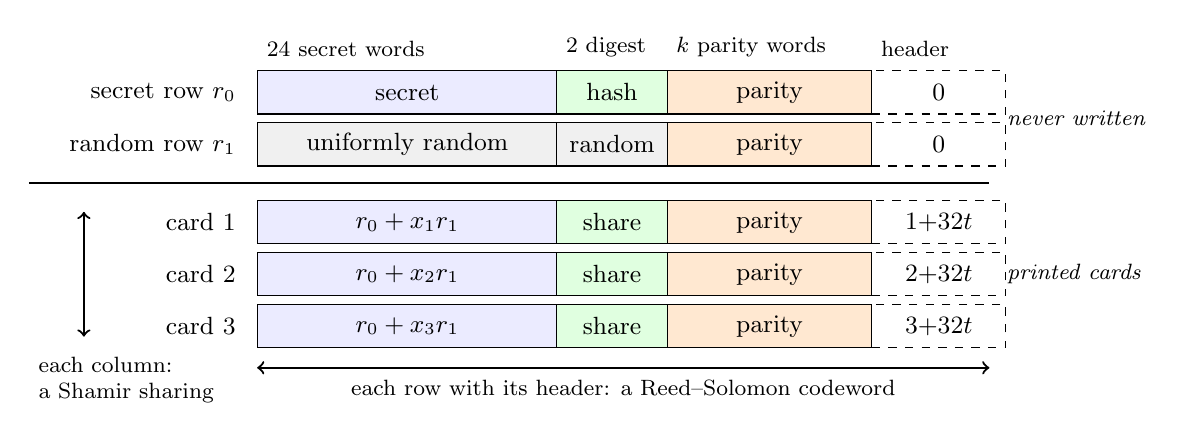
\begin{tikzpicture}[x=1cm,y=0.66cm,font=\small,
  cell/.style={draw,minimum height=0.55cm,inner sep=1pt,anchor=west},
  data/.style={cell,minimum width=3.8cm,fill=blue!8},
  dig/.style={cell,minimum width=1.4cm,fill=green!12},
  par/.style={cell,minimum width=2.6cm,fill=orange!18},
  hdr/.style={cell,minimum width=1.7cm,dashed}]
\node[anchor=south west,font=\footnotesize] at (0,0.5) {24 secret words};
\node[anchor=south west,font=\footnotesize] at (3.8,0.5) {2 digest};
\node[anchor=south west,font=\footnotesize] at (5.2,0.5) {$k$ parity words};
\node[anchor=south west,font=\footnotesize] at (7.8,0.5) {header};
\node[anchor=east] at (-0.15,0) {secret row $r_0$};
\node[data] at (0,0) {secret};
\node[dig] at (3.8,0) {hash};
\node[par] at (5.2,0) {parity};
\node[hdr] at (7.8,0) {0};
\node[anchor=east] at (-0.15,-1) {random row $r_1$};
\node[data,fill=gray!12] at (0,-1) {uniformly random};
\node[dig,fill=gray!12] at (3.8,-1) {random};
\node[par] at (5.2,-1) {parity};
\node[hdr] at (7.8,-1) {0};
\draw[thick] (-2.9,-1.75) -- (9.3,-1.75);
\node[anchor=west,font=\footnotesize\itshape] at (9.4,-0.5) {never written};
\node[anchor=west,font=\footnotesize\itshape] at (9.4,-3.5) {printed cards};
\foreach \i/\y in {1/-2.5,2/-3.5,3/-4.5}{
  \node[anchor=east] at (-0.15,\y) {card \i};
  \node[data] at (0,\y) {$r_0 + x_{\i} r_1$};
  \node[dig] at (3.8,\y) {share};
  \node[par] at (5.2,\y) {parity};
  \node[hdr] at (7.8,\y) {$\i{+}32t$};
}
\draw[<->,thick] (-2.2,-2.3) -- (-2.2,-4.7);
\node[anchor=north west,font=\footnotesize,align=left] at (-2.9,-4.9) {each column:\\ a Shamir sharing};
\draw[<->,thick] (0,-5.3) -- (9.3,-5.3);
\node[anchor=north,font=\footnotesize] at (4.65,-5.35) {each row with its header: a Reed--Solomon codeword};
\end{tikzpicture}

\caption{Grid shares for $t=2$, $n=3$. Each card, extended by its unprinted
header, is a Reed--Solomon codeword, so it can be repaired alone. Each word
position is a Shamir sharing across cards, so any $t$ cards determine it and
spare cards expose a wrong entry.}
\label{fig:grid}
\end{figure}

Since $u$ is zero on the data words, the term $h_i u$ changes only the parity
words of a card, by a known multiple of a fixed vector. Subtracting it from a
card whose number is known leaves the \emph{stripped} card
$y_i=\sum_d x_i^d r_d$, restricted to its $W$ printed positions.

\begin{proposition}
\label{prop:grid}
(a) Every $c_i$ is a valid codeword of length $W+1$. As a consequence the
printed words of two different cards with the same number differ in at least
$k+1$ positions, and of two cards with different numbers in at least $k$.
(b) Any $t$ stripped cards determine $r_0$.
(c) Any $t-1$ cards are statistically independent of the data words of $r_0$.
(d) The stripped cards of any $m\ge t$ holders, read as an $m\times W$ array,
differ between two distinct dealings in at least $(k+1)(m-t+1)$ entries.
\end{proposition}

\begin{proof}
(a) The syndromes are linear and $r_0,\dots,r_{t-1},u$ are valid. Two codewords
differ in at least $k+1$ of their $W+1$ positions, and the header is one
position.
(b) In each column the stripped values are evaluations of a polynomial of
degree below $t$ at distinct points; interpolation at $0$ gives the entry of
$r_0$.
(c) In each data column this is Shamir's scheme~\citep{shamir1979how} with
independent randomness per column. The parity words and header of a card are
functions of its data words, its number and $t$, and add nothing.
(d) The array is a codeword of the product of a length-$m$ Reed--Solomon code
of distance $m-t+1$~\citep{mceliece1981sharing} with a row code of distance
$k+1$; distances of a product multiply~\citep{elias1954error}.
\end{proof}

Part (a) is why a legible card number matters: a card whose number is known has
the full distance $k+1$, and one whose number must be inferred has $k$. Part
(d) bounds what any decoder can promise when numbers are known: up to
$\lfloor((k+1)(m-t+1)-1)/2\rfloor$ wrong words \emph{anywhere} among the $m$
cards leave the dealing uniquely determined. For 30-word cards with $k=4$ that
is 2 words with two cards of a 2-of-3 set, 4 with all three, and 7 with all
five cards of a 3-of-5 set. Our decoder (Section~\ref{sec:decoder}) is
iterative and is not shown to correct every pattern within this bound.

\subsection{Reading the header}

If the number written on a card is legible, $h_i$ is known and is supplied to
the repair procedure of Section~\ref{sec:parity} as a known symbol. If it is not, the header is treated as one
more unreadable symbol; when that leaves too little parity for a unique
repair, the decoder tries each of the 31 possible numbers as if known and keeps
the candidates of least cost. The header costs no written words. A card entered with the wrong number has
one wrong symbol, the header, which the repair procedure corrects like any
other wrong word and reports; the number it settles on is the one consistent
with the card's words.

\subsection{The digest}
\label{sec:digest}

A linear code cannot tell a correct reconstruction from a consistent wrong one.
With exactly $t$ cards, every combination of valid cards interpolates to
\emph{some} valid row, including when one card comes from a different dealing.
As SLIP39 does~\citep{slip39}, we therefore share a hash of the secret along
with it. Let $H$ be the SHA-256 hash of the ASCII string
\code{bip39-parity/digest} followed by each secret word as two big-endian
bytes. Digest word $j$ ($j=0,\dots,g-1$) is the low 11 bits of the 16-bit
big-endian integer formed by bytes $2j$ and $2j+1$ of $H$. For the mnemonic of
23 times \code{abandon} followed by \code{art}, the two digest words are
\code{siege} and \code{say}.

A reconstruction is accepted only if its digest words match its secret words.
If SHA-256 output is modelled as uniformly random, a wrong candidate passes
with probability $2^{-11g}$; we use $g=2$, so $2^{-22}$ per candidate. A holder
who alters a card without knowing the secret faces the same odds on each
attempt.

The digest is shared like every other data word, so by
Proposition~\ref{prop:grid}(c) fewer than $t$ cards learn nothing about it.

\subsection{Decoding}
\label{sec:decoder}

\begin{enumerate}
\item \emph{Rows.} Repair each card alone as in Section~\ref{sec:parity},
  without the BIP39 filter, which does not apply to share words. A card with a
  unique repair is \emph{confirmed} and stripped of its header term. A card
  with none, but with a legible number and the right count of words, is kept
  as unconfirmed evidence. Other cards are set aside.
\item \emph{Columns.} For each word position, find the polynomial of degree
  below $t$ that agrees with the most cards, using confirmed cards alone when
  there are at least $t$. With exactly $t$ values the column is taken as given;
  with more, it is settled only if at least $t+1$ values agree and no rival
  polynomial ties.
\item \emph{Iterate.} Settled columns supply words to unconfirmed cards, which
  are then decoded again as rows; newly confirmed cards settle more columns.
\item \emph{Rescue.} If confirmed cards are one short of $t$, $k\ge 3$, and at
  most 14 columns are unsettled, guess a set of 3 to $k$ of those columns as
  the error positions of an unconfirmed card, mark them unreadable, decode, and
  accept only if every guessed position then agrees with another card.
\item \emph{Check.} Interpolate the secret row from the settled columns, decode
  it as a row (its own parity may fill columns that did not settle), and test
  the digest. If that fails and more than $t$ cards are confirmed, test the
  reconstruction from each subset of $t$ of them, which finds the right
  subset when one card does not belong. If nothing passes, refuse.
\end{enumerate}

With $m$ confirmed cards step 5 tests at most $\binom{m}{t}+1$ candidates, so
the chance of accepting a wrong secret is at most
$\bigl(\binom{m}{t}+1\bigr)2^{-22}$: about $2.6\times10^{-6}$ for $m=5$,
$t=3$. This is a design figure; our experiments are too small to test it.

\subsection{Why not split one long phrase?}
\label{sec:ramp}

A tempting shortcut is to encode once with large $k$ and hand each party a
segment, since any $N$ of the $N+k$ words recover the rest. This is a ramp
scheme, not threshold sharing: with no fresh randomness, every word a party
holds is 11 bits of constraint on the secret. A party holding $q$ words of a
24-word phrase faces $264-11q$ unknown bits, so a 12-word segment leaves 132
bits of the phrase, or 124 bits of entropy after the 8-bit BIP39 checksum. That
is beyond exhaustive search, but it is half the secret rather than none of it,
it shrinks with every further word, and two segment holders together have
everything. Grid shares cost longer cards and give the property people expect
from Shamir: below the threshold, nothing.

\section{Experiments}
\label{sec:experiments}

\subsection{Setup}

The implementation is compiled to native code through Lean's C backend and
depends only on the Lean core library. Two harnesses inject faults:
\code{tests} for single phrases and \code{gridtests} for grids. Each trial
draws fresh entropy, encodes or deals, damages the written words, and decodes.
For grids an outcome is \emph{correct} (the original secret is returned),
\emph{wrong} (a different secret is returned), or \emph{refused}. For single
phrases the outcomes are \emph{unique} (the original phrase is the only
candidate), \emph{ambiguous} (it is one of several), \emph{wrong} (only other
phrases are offered) and \emph{refused}. The random generator has a fixed seed,
so every table is reproduced exactly by the commands in
Section~\ref{sec:repro}.

Grids use 24 secret words, 2 digest words and $k=4$ unless stated. The faults:
\begin{itemize}
\item a \emph{word error} replaces a word by a different uniformly random
  word, independently per word at the stated rate;
\item a \emph{burn} makes a run of consecutive words unreadable;
\item a \emph{swap} exchanges two randomly chosen words of a card;
\item a \emph{dropped word} removes one word from a card, with probability
  one half per card;
\item a \emph{foreign} card is the same-numbered card of an unrelated dealing,
  and a \emph{garbage} card is random words;
\item with \emph{numbers illegible}, no card number is given to the decoder.
\end{itemize}
Card numbers are otherwise given correctly. We compare five ways of using the
same cards:
\begin{itemize}
\item \emph{Checksum only}: a card counts only if it is exactly valid as
  written; the first $t$ such cards are interpolated. This models a per-share
  detection checksum.
\item \emph{Card parity}: each card is repaired alone; the first $t$ repaired
  cards are interpolated.
\item \emph{Card parity + digest}: each card is repaired alone; the first
  subset of $t$ repaired cards whose reconstruction passes the digest is
  used. This is per-share correction with the mix-up defence of deployed
  formats, and no decoding across cards.
\item \emph{Grid, no digest}: joint decoding as in
  Section~\ref{sec:decoder}, accepting the secret row on its parity alone.
\item \emph{Grid}: the full decoder of Section~\ref{sec:decoder}, joint
  decoding with the digest.
\end{itemize}
A percentage from 400 trials has a 95\% confidence half-width of at most 4.9
points; from 300, 250 and 200 trials, 5.7, 6.2 and 6.9 points. We do not
interpret smaller differences. The harness truncates percentages to one
decimal, so a row's entries can sum to 99.9. Where the same configuration appears in two
tables it was run twice with different random draws, and the two values differ
within these margins.

\subsection{Single phrases}

Table~\ref{tab:single} gives the fraction of trials in which the original
phrase was the unique repair, without and with the BIP39 checksum as a filter.
Everything inside the capacity~\eqref{eq:cap} is repaired, as it must be. The
informative rows are the edits. With the filter, two parity words repair a
swap or a dropped word, three repair two dropped words or a wrong word plus a
dropped word, and four repair any two wrong words. Without the filter the
same holds from one parity word more: at $k=2$ a swap is the unique repair in
84.5--96.5\% of trials and otherwise ambiguous. Faults beyond the capacity
(two wrong words at $k\le3$; a wrong word plus a dropped word at $k=2$) were
refused, apart from 0.5--1.5\% of unfiltered trials at $k=2$ in which a single
wrong phrase was offered (footnote in the table). With the filter, or with
$k\ge 3$, no trial was wrong.

\begin{table}[!htb]
\centering
\caption{Single phrases: percentage of 200 trials in which the original phrase
was the unique repair, without / with the BIP39 checksum filter. ``Refused''
means no candidate was offered, in every trial with the filter and in every
trial without it except as footnoted.}
\label{tab:single}
\small
\begin{tabular}{lcccccc}
\toprule
Fault & 12+2 & 12+3 & 12+4 & 24+2 & 24+3 & 24+4 \\
\midrule
1 wrong word & 100 / 100 & 100 / 100 & 100 / 100 & 100 / 100 & 100 / 100 & 100 / 100 \\
2 unreadable words & 100 / 100 & 100 / 100 & 100 / 100 & 100 / 100 & 100 / 100 & 100 / 100 \\
adjacent words swapped & 94 / 100 & 100 / 100 & 100 / 100 & 87 / 100 & 100 / 100 & 100 / 100 \\
any 2 words swapped & 96.5 / 100 & 100 / 100 & 100 / 100 & 84.5 / 99.5 & 100 / 100 & 100 / 100 \\
1 dropped word & 99 / 100 & 100 / 100 & 100 / 100 & 99.5 / 100 & 100 / 100 & 100 / 100 \\
1 extra word & 100 / 100 & 100 / 100 & 100 / 100 & 100 / 100 & 100 / 100 & 100 / 100 \\
2 dropped words & 0 / 1 & 96 / 99.5 & 100 / 100 & 0 / 30 & 82 / 100 & 100 / 100 \\
1 wrong + 1 dropped & refused$^{a}$ & 92.5 / 99.5 & 100 / 100 & refused$^{a}$ & 76 / 99.5 & 100 / 100 \\
2 wrong words & refused & refused & 100 / 100 & refused$^{a}$ & refused & 100 / 100 \\
\bottomrule
\multicolumn{7}{l}{\footnotesize $^{a}$ Without the filter, a single wrong phrase
was offered in 0.5\% (12+2) or 1.5\% (24+2) of trials.}
\end{tabular}
\end{table}

\subsection{Grids}

Table~\ref{tab:grid} and Figure~\ref{fig:rates} give the main results.

\begin{table}[!htb]
\centering
\caption{Grid shares, 30-word cards ($k=4$), 400 trials per cell. Entries are
the percentage of trials that returned the correct secret, for 2-of-3 / 3-of-5.
A bracket gives the percentage that returned a \emph{wrong} secret where that
is not zero. All other trials were refused, so 0 with no bracket means every
trial was refused.}
\label{tab:grid}
\footnotesize
\setlength{\tabcolsep}{2.5pt}
\begin{tabular}{lccccc}
\toprule
 & Checksum & Card & Card parity & Grid, & \\
Damage & only & parity & + digest & no digest & Grid \\
\midrule
\multicolumn{6}{l}{\emph{All $n$ cards at hand}}\\
1\% of words wrong & 80.7 / 89.2 & 100 / 100 & 100 / 100 & 100 / 100 & 100 / 100 \\
3\% of words wrong & 33 / 33.2 & 99.2 / 99.7 & 99.2 / 99.7 & 99.7 / 100 & 99.7 / 100 \\
5\% of words wrong & 12.7 / 7 & 93.5 / 95.5 & 93.5 / 95.5 & 96.7 / 100 & 96.7 / 100 \\
10\% of words wrong & 1 / 0 & 40.7 / 30.5 & 40.7 / 30.5 & 61.2 / 99.5 & 61.2 / 99.5 \\
5 words burnt per card & 0 / 0 & 0 / 0 & 0 / 0 & 89.7 / 98.2 & 89.7 / 98.2 \\
8 words burnt per card & 0 / 0 & 0 / 0 & 0 / 0 & 34.7 / 59.5 & 34.7 / 59.5 \\
one swap per card & 0 / 0 & 100 / 100 & 100 / 100 & 100 / 100 & 100 / 100 \\
one swap per card, 3\% wrong & 0 / 0 & 86.2 / 92.7 & 86.2 / 92.7 & 92.5 / 100 & 92.5 / 100 \\
dropped words, 3\% wrong & 10.2 / 7 & 94.5 / 98.2 & 94.5 / 98.2 & 94.7 / 98.2 & 94.7 / 98.2 \\
numbers illegible, 3\% wrong & 36 / 34 & 98 / 99.7 & 98 / 99.7 & 98 / 99.7 & 98 / 99.7 \\
one garbage card, 1\% wrong & 52.7 / 73 & 99.2 / 100 & 99.2 / 100 & 99.2 / 100 & 99.2 / 100 \\
one card is foreign & 33 / 40.2 {\scriptsize[67 / 59.7]} & 33 / 40.2 {\scriptsize[67 / 59.7]} & 100 / 100 & 0 / 100 & 100 / 100 \\
\midrule
\multicolumn{6}{l}{\emph{Only $t$ cards at hand}}\\
1\% of words wrong & 57.2 / 38 & 99.5 / 99.7 & 99.5 / 99.7 & 99.5 / 99.7 & 99.5 / 99.7 \\
3\% of words wrong & 16.7 / 5.5 & 87.7 / 84.5 & 87.7 / 84.5 & 87.7 / 84.5 & 87.7 / 84.5 \\
5\% of words wrong & 3.2 / 0.5 & 62 / 50.7 {\scriptsize[0 / 0.2]} & 62 / 50.7 & 62 / 50.7 {\scriptsize[0 / 0.2]} & 62 / 50.7 \\
one swap per card & 0 / 0 & 100 / 100 & 100 / 100 & 100 / 100 & 100 / 100 \\
one card is foreign & 0 / 0 {\scriptsize[100 / 100]} & 0 / 0 {\scriptsize[100 / 100]} & 0 / 0 & 0 / 0 {\scriptsize[100 / 100]} & 0 / 0 \\
\bottomrule
\end{tabular}
\end{table}

\begin{figure}[!htb]
\centering
% Correct recoveries vs per-word error rate.
% Generated by figures/src/tables.py from refs/experiments/grid-main-k4.txt
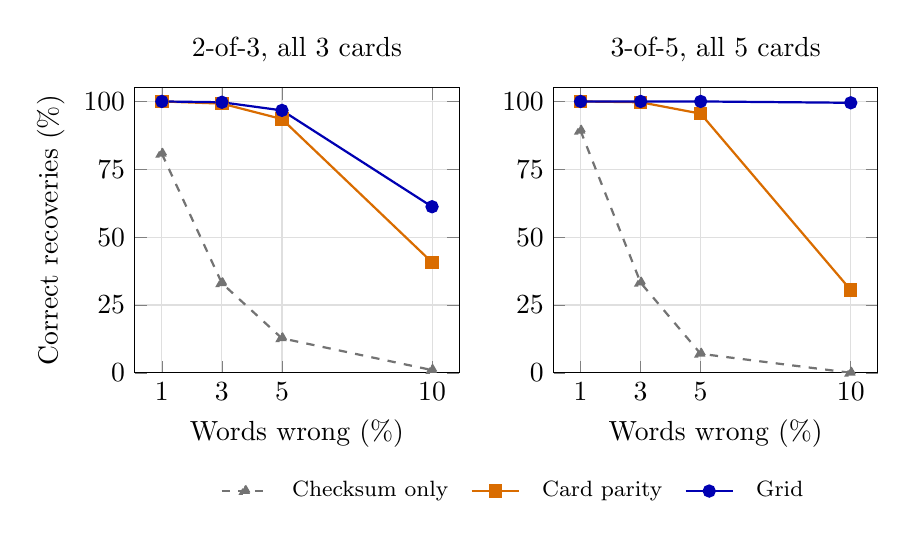
\begin{tikzpicture}
\begin{groupplot}[
  group style={group size=2 by 1, horizontal sep=1.2cm, ylabels at=edge left},
  width=0.47\linewidth, height=5.2cm,
  xlabel={Words wrong (\%)}, ylabel={Correct recoveries (\%)},
  xtick={1,3,5,10}, ymin=0, ymax=105, ytick={0,25,50,75,100},
  grid=major, grid style={gray!25},
  legend style={font=\footnotesize, draw=none, fill=none, legend columns=3, column sep=6pt, at={(-0.12,-0.34)}, anchor=north},
  every axis plot/.append style={thick, mark size=2pt}]
\nextgroupplot[title={2-of-3, all 3 cards}]
\addplot[color=black!55, mark=triangle*, dashed] coordinates {(1,80.7) (3,33.0) (5,12.7) (10,1.0)};
\addplot[color=orange!85!black, mark=square*] coordinates {(1,100.0) (3,99.2) (5,93.5) (10,40.7)};
\addplot[color=blue!70!black, mark=*] coordinates {(1,100.0) (3,99.7) (5,96.7) (10,61.2)};
\nextgroupplot[title={3-of-5, all 5 cards}]
\addplot[color=black!55, mark=triangle*, dashed] coordinates {(1,89.2) (3,33.2) (5,7.0) (10,0.0)};
\addlegendentry{Checksum only}
\addplot[color=orange!85!black, mark=square*] coordinates {(1,100.0) (3,99.7) (5,95.5) (10,30.5)};
\addlegendentry{Card parity}
\addplot[color=blue!70!black, mark=*] coordinates {(1,100.0) (3,100.0) (5,100.0) (10,99.5)};
\addlegendentry{Grid}
\end{groupplot}
\end{tikzpicture}

\caption{Correct recoveries with all cards at hand as the per-word error rate
grows (Table~\ref{tab:grid}, 400 trials per point). With one spare card
(2-of-3) joint decoding matches per-card repair up to 5\% and gains 20 points
at 10\%. With two spare cards (3-of-5) it nearly removes the dependence on
the error rate.}
\label{fig:rates}
\end{figure}

\emph{Spare cards turn into error correction.} With all five cards of a 3-of-5
set and one word in ten wrong, the grid decoder recovers 99.5\% of secrets;
repairing cards one at a time recovers 31\%, because three of the five cards
must each have at most two wrong words. With the single spare card of a 2-of-3
set the gain at that rate is smaller, 61\% against 41\%, and below 5\% the two
methods are within sampling error.

\emph{Runs of unreadable words.} Five consecutive unreadable words exceed what
$k=4$ can fill, so no card repairs alone and every per-card method recovers
nothing. The grid decoder recovers 90\% (2-of-3) and 98\% (3-of-5), because
the burns fall in different columns on different cards.

\emph{Swaps and dropped words.} One swap on every card is repaired by every card
on its own, with all cards or with exactly $t$: 100\% in each case, where a
detection checksum recovers nothing. With 3\% of words also wrong, per-card
repair falls to 86\% (2-of-3) and 93\% (3-of-5), since a swap leaves room for
only one further wrong word at $k=4$, and joint decoding brings that back to
92.5\% and 100\%. Dropped words gain nothing from joint decoding (94.7\% and
98.2\%, equal to per-card repair within error), because a card that is short
and does not repair alone is set aside.

\emph{Wrong cards: the digest matters most when spares are few.} When one
card is foreign, per-card methods without a digest return a wrong secret
whenever that card is among the first $t$ used (60--67\% of trials). Joint
decoding without a digest outvotes the foreign card when there are two spare
cards (100\% for 3-of-5), refuses when there is one (2-of-3), and returns a
wrong secret every time when there is none. Adding the digest to either
approach removes every wrong answer and recovers whenever a spare card
exists. The defence against mixed-up cards is therefore the digest, as in
deployed formats, and not joint decoding. With exactly $t$ cards and one
foreign, no method can recover, and the two with a digest refuse.

\emph{Illegible numbers.} With no card numbers and 3\% of words wrong, the grid
decoder recovers 98\% (2-of-3) and 99.7\% (3-of-5), against 99.7\% and
100\% with legible numbers: inferring the header costs little.

\emph{Wrong answers.} A card with more wrong words than its parity can
correct occasionally repairs to a different valid card. This happened once,
in the 3-of-5 row with exactly $t$ cards and 5\% of words wrong, where both
methods without a digest returned a wrong secret (the bracketed 0.2). The digest
turned that trial into a refusal. Across all 31{,}600 grid trials in this paper the two
methods with a digest returned no wrong secret. Pooled, that bounds the rate of
wrong answers under these fault models below about $10^{-4}$ at 95\% confidence
(if the rate were higher, at least one wrong answer would have been
expected with that confidence), and below 0.75\% for any single 400-trial cell. It says
nothing about fault patterns we did not inject.

\subsection{With exactly $t$ cards, only $k$ helps}

The lower half of Table~\ref{tab:grid} is the scheme's weak case. With exactly
$t$ cards there are no spare rows, the grid decoder equals per-card repair, and
\emph{every} card must repair. At 3\% wrong words, $k=4$ recovers 88\% (2-of-3)
and 85\% (3-of-5). Table~\ref{tab:k} shows that the remedy is more parity per
card: $k=8$ restores 99\% at the cost of four more written words.

\begin{table}[!htb]
\centering
\caption{Only $t$ cards at hand: percentage correct for 2-of-3 / 3-of-5 as the
number of parity words per card grows ($k=4$: 400 trials; $k=6,8$: 300
trials), grid decoder. It returned no wrong secret.}
\label{tab:k}
\small
\begin{tabular}{lccc}
\toprule
Words wrong & $k=4$ (30 words) & $k=6$ (32 words) & $k=8$ (34 words) \\
\midrule
3\% & 87.7 / 84.5 & 95.6 / 94 & 99 / 99 \\
5\% & 62 / 50.7 & 83.6 / 78.6 & 95.6 / 94.6 \\
\bottomrule
\end{tabular}
\end{table}

\section{Custody Arrangements}
\label{sec:scenarios}

The number of cards a group can bring together decides which half of
Table~\ref{tab:grid} applies. Table~\ref{tab:scen} works through three
arrangements.

\begin{table}[!htb]
\centering
\caption{Percentage of correct recoveries by number of cards brought together
($k=4$, 250 trials per cell, grid decoder; no trial returned a wrong secret,
so 0 means every trial was refused). The first three columns are word error
rates. ``Garbage'' replaces one card by random words, with 1\% word errors on
the rest; ``foreign'' replaces one card by a card of another dealing;
``burnt'' is five consecutive unreadable words on every card.}
\label{tab:scen}
\small
\begin{tabular}{llcccccc}
\toprule
Scheme & Cards & 1\% & 3\% & 5\% & Garbage & Foreign & Burnt \\
\midrule
3-of-6 & 3 & 99.2 & 82.4 & 50.8 & 0 & 0 & 0 \\
 & 4 & 100 & 98.4 & 94 & 100 & 100 & 76.8 \\
 & 6 & 100 & 100 & 100 & 100 & 100 & 100 \\
\midrule
3-of-5 & 3 & 99.6 & 83.2 & 54.8 & 0 & 0 & 0 \\
 & 4 & 100 & 98.8 & 89.6 & 99.6 & 100 & 72 \\
 & 5 & 100 & 100 & 100 & 100 & 100 & 98 \\
\midrule
4-of-9 & 4 & 98.4 & 73.6 & 40 & 0 & 0 & 0 \\
 & 5 & 100 & 99.2 & 87.6 & 96.8 & 100 & 62.8 \\
\bottomrule
\end{tabular}
\end{table}

\paragraph{Three people, two cards each (3-of-6).}
One person holds two cards and learns nothing. Any two people hold four: one
more than the threshold, which is the ``4 cards'' row. The pair can lose or
ruin one card and still recover, can identify a card that does not belong, and
recover 98\% of the time at a 3\% word error rate. All three together recovered
in every trial of every fault we injected. The cost of the convenience is on
the theft side: one person plus any single stolen card reaches the threshold.

\paragraph{An owner with three cards and two backup holders (3-of-5).}
The owner can recover alone, but with exactly $t$ cards and therefore no
margin: 83\% at a 3\% error rate, and nothing if one card is lost or burnt. One
backup holder's card restores the margin (98.8\%). The two backup holders
together hold two cards and learn nothing. Since the owner's three cards are a
complete key, they should be stored in separate places, and an owner who
expects to recover alone should use $k=6$ or $k=8$ (Table~\ref{tab:k}).

\paragraph{Weighted inheritance (4-of-9).}
An owner holds four cards, an executor two, and three heirs one each. The owner
recovers alone; after the owner's death the executor and any two heirs reach
four, and with the third heir five. The heirs alone hold three and learn
nothing, and so does the executor alone. Weights come for free because cards
are interchangeable evaluations.

\paragraph{The general rule.}
Plan for one more card than the threshold to be present at recovery. A spare
card moves an arrangement from the lower half of Table~\ref{tab:grid} to the
upper half, and it is the only way to survive a card that is wrong as a whole.

\section{Discussion}
\label{sec:limits}

\paragraph{Security.}
Secrecy below the threshold is information-theoretic
(Proposition~\ref{prop:grid}c) and depends on the $t-1$ random rows being
uniform; the dealer must use a cryptographic random source. Parity reveals
nothing about the secret, but a single card does reveal the threshold and its
own number. The digest protects against accidents and against a holder who
alters a card without knowing the secret. It is not a defence against a dealer
who cheats or a holder who already knows the secret; verifiable sharing
addresses those~\citep{rabin1989verifiable} and is out of scope. Redundancy
does not help an attacker who has $t$ cards, and does not weaken the secret:
parity words are public functions of words the holder already has.

\paragraph{Limits of the evidence.}
(1) Word error rates of 1--10\% are an assumption. The study we cite measures
recall from memory, not copying, and real errors are not uniform: people
confuse similar words. (2) Faults within a card were independent except for
burns. (3) The implementation is tested, not verified; its unit tests cover
the field axioms, SHA-256 and BIP39 reference vectors, and decoding within
capacity for $k=1,\dots,8$, but no theorem about the decoder is proved in
Lean. (4) The grid decoder is a heuristic. It sets aside a card with dropped
words that does not repair alone instead of using it as evidence, and the
rescue step applies only when confirmed cards are one short.
Proposition~\ref{prop:grid}(d) says a better decoder exists for some
patterns. (5) The edit search is bounded at three dropped or extra words and
one swap.

\paragraph{Choosing $k$.}
The measurements suggest $k=4$ when a spare card will normally be present and
$k=6$ or more when recovery from exactly $t$ cards is the expected path. For an
unshared 24-word phrase, $k=3$ covers every single edit and $k=4$ any two wrong
words.

\paragraph{Open directions.}
A packed variant that shares two secret words per column would give 12-word
cards for a 24-word secret at the price of ramp-style leakage between one and
$t$ cards. Measuring real transcription errors would replace our assumed rates.
The Lean sources are a natural basis for a verified decoder.

\section{Reproducibility}
\label{sec:repro}

All numbers come from the source tree that accompanies this paper (repository
\code{bip39-parity}), built with \code{lake build} under the Lean toolchain
\code{v4.36.0}. The tree is not yet published at a public address. To pin the
version, the file \code{refs/experiments/README.txt} distributed with the paper
sources lists the SHA-256 of every source file used. The harness outputs are
stored verbatim in the same folder, each headed by its command:
\begin{itemize}
\item Table~\ref{tab:single}: \code{lake exe tests 200}
  (\code{single-phrase.txt})
\item Table~\ref{tab:grid} and Figure~\ref{fig:rates}:
  \code{lake exe gridtests 400} (\code{grid-main-k4.txt})
\item Table~\ref{tab:k} (\code{grid-minimal-k6.txt} and \code{-k8.txt}):\\
  \code{lake exe gridtests 300 "only t cards," 6}, and the same with \code{8}
\item Table~\ref{tab:scen}, one command per scheme
  (\code{scenario-*.txt}):\\
  \code{lake exe gridtests custom 250 4 3 6 3 4 6}\\
  \code{lake exe gridtests custom 250 4 3 5 3 4 5}\\
  \code{lake exe gridtests custom 250 4 4 9 4 5}
\end{itemize}
The random seed is fixed in the harness (39). The trial total counts every row
of the six grid files, including rows that no table prints. The command-line tool exposes the scheme directly: the
subcommands \code{encode}, \code{check} and \code{repair} of \code{parity39}
handle single phrases, and \code{split} and \code{combine} handle grids.

\section{Conclusion}
\label{sec:conclusion}

Because a BIP39 word is a field element, a mnemonic can carry Reed--Solomon
parity in its own alphabet, and Shamir shares of such mnemonics are codewords
of the same kind. With the BIP39 checksum as a filter, two parity words repair a swap or a
dropped word, and four repair any two wrong words. Shared as a grid, cards repair themselves and each
other: with spare cards the decoder recovered from word error rates and runs
of unreadable words that defeat repair card by card, and with the digest it
returned no wrong secret in 31{,}600 trials. With no spare card, reliability
comes only from parity per card, and the arrangement should be chosen with
that in mind.

\bibliographystyle{plainnat}
\bibliography{refs}

\end{document}
